\documentclass[a4paper,12pt,twoside]{memoir}

\usepackage{longtable}
\usepackage{eurosym}
\usepackage{listings}
\usepackage[spanish]{algorithm2e}

% Castellano
\usepackage[spanish,es-tabla]{babel}
\selectlanguage{spanish}
\usepackage[utf8]{inputenc}
\usepackage[T1]{fontenc}
\usepackage{lmodern} % scalable font
\usepackage{microtype}
\usepackage{placeins}

\RequirePackage{booktabs}
\RequirePackage[table]{xcolor}
\RequirePackage{xtab}
\RequirePackage{multirow}

% Links
\PassOptionsToPackage{hyphens}{url}\usepackage[colorlinks]{hyperref}
\hypersetup{
	allcolors = {red}
}

% Ecuaciones
\usepackage{amsmath}

% Rutas de fichero / paquete
\newcommand{\ruta}[1]{{\sffamily #1}}

% Párrafos
\nonzeroparskip

% Huérfanas y viudas
\widowpenalty100000
\clubpenalty100000

% Evitar solapes en el header
\nouppercaseheads

% Imagenes
\usepackage{graphicx}
\newcommand{\imagen}[2]{
	\begin{figure}[!h]
		\centering
		\includegraphics[width=0.9\textwidth]{#1}
		\caption{#2}\label{fig:#1}
	\end{figure}
	\FloatBarrier
}

\newcommand{\imagenflotante}[2]{
	\begin{figure}%[!h]
		\centering
		\includegraphics[width=0.9\textwidth]{#1}
		\caption{#2}\label{fig:#1}
	\end{figure}
}



% El comando \figura nos permite insertar figuras comodamente, y utilizando
% siempre el mismo formato. Los parametros son:
% 1 -> Porcentaje del ancho de página que ocupará la figura (de 0 a 1)
% 2 --> Fichero de la imagen
% 3 --> Texto a pie de imagen
% 4 --> Etiqueta (label) para referencias
% 5 --> Opciones que queramos pasarle al \includegraphics
% 6 --> Opciones de posicionamiento a pasarle a \begin{figure}
\newcommand{\figuraConPosicion}[6]{%
  \setlength{\anchoFloat}{#1\textwidth}%
  \addtolength{\anchoFloat}{-4\fboxsep}%
  \setlength{\anchoFigura}{\anchoFloat}%
  \begin{figure}[#6]
    \begin{center}%
      \Ovalbox{%
        \begin{minipage}{\anchoFloat}%
          \begin{center}%
            \includegraphics[width=\anchoFigura,#5]{#2}%
            \caption{#3}%
            \label{#4}%
          \end{center}%
        \end{minipage}
      }%
    \end{center}%
  \end{figure}%
}

%
% Comando para incluir imágenes en formato apaisado (sin marco).
\newcommand{\figuraApaisadaSinMarco}[5]{%
  \begin{figure}%
    \begin{center}%
    \includegraphics[angle=90,height=#1\textheight,#5]{#2}%
    \caption{#3}%
    \label{#4}%
    \end{center}%
  \end{figure}%
}
% Para las tablas
\newcommand{\otoprule}{\midrule [\heavyrulewidth]}
%
% Nuevo comando para tablas pequeñas (menos de una página).
\newcommand{\tablaSmall}[5]{%
 \begin{table}
  \begin{center}
   \rowcolors {2}{gray!35}{}
   \begin{tabular}{#2}
    \toprule
    #4
    \otoprule
    #5
    \bottomrule
   \end{tabular}
   \caption{#1}
   \label{tabla:#3}
  \end{center}
 \end{table}
}

%
%Para el float H de tablaSmallSinColores
\usepackage{float}

%
% Nuevo comando para tablas pequeñas (menos de una página).
\newcommand{\tablaSmallSinColores}[5]{%
 \begin{table}[H]
  \begin{center}
   \begin{tabular}{#2}
    \toprule  
    #4
    \otoprule
    #5
    \bottomrule
   \end{tabular}
   \caption{#1}
   \label{tabla:#3}
  \end{center}
 \end{table}
}

\newcommand{\tablaApaisadaSmall}[5]{%
\begin{landscape}
  \begin{table}
   \begin{center}
    \rowcolors {2}{gray!35}{}
    \begin{tabular}{#2}
     \toprule
     #4
     \otoprule
     #5
     \bottomrule
    \end{tabular}
    \caption{#1}
    \label{tabla:#3}
   \end{center}
  \end{table}
\end{landscape}
}
 
%
% Nuevo comando para tablas grandes con cabecera y filas alternas coloreadas en gris.
\newcommand{\tabla}[6]{%
  \begin{center}
    \tablefirsthead{
      \toprule
      #5
      \otoprule
    }
    \tablehead{
      \multicolumn{#3}{l}{\small\sl continúa desde la página anterior}\\
      \toprule
      #5
      \otoprule
    }
    \tabletail{
      \hline
      \multicolumn{#3}{r}{\small\sl continúa en la página siguiente}\\
    }
    \tablelasttail{
      \hline
    }
    \bottomcaption{#1}
    \rowcolors {2}{gray!35}{}
    \begin{xtabular}{#2}
      #6
      \bottomrule
    \end{xtabular}
    \label{tabla:#4}
  \end{center}
}

%
% Nuevo comando para tablas grandes con cabecera.
\newcommand{\tablaSinColores}[6]{%
  \begin{center}
    \tablefirsthead{
      \toprule
      #5
      \otoprule
    }
    \tablehead{
      \multicolumn{#3}{l}{\small\sl continúa desde la página anterior}\\
      \toprule
      #5
      \otoprule
    }
    \tabletail{
      \hline
      \multicolumn{#3}{r}{\small\sl continúa en la página siguiente}\\
    }
    \tablelasttail{
      \hline
    }
    \bottomcaption{#1}
    \begin{xtabular}{#2}
      #6
      \bottomrule
    \end{xtabular}
    \label{tabla:#4}
  \end{center}
}

%
% Nuevo comando para tablas grandes sin cabecera.
\newcommand{\tablaSinCabecera}[5]{%
  \begin{center}
    \tablefirsthead{
      \toprule
    }
    \tablehead{
      \multicolumn{#3}{l}{\small\sl continúa desde la página anterior}\\
      \hline
    }
    \tabletail{
      \hline
      \multicolumn{#3}{r}{\small\sl continúa en la página siguiente}\\
    }
    \tablelasttail{
      \hline
    }
    \bottomcaption{#1}
  \begin{xtabular}{#2}
    #5
   \bottomrule
  \end{xtabular}
  \label{tabla:#4}
  \end{center}
}



\definecolor{cgoLight}{HTML}{EEEEEE}
\definecolor{cgoExtralight}{HTML}{FFFFFF}

%
% Nuevo comando para tablas grandes sin cabecera.
\newcommand{\tablaSinCabeceraConBandas}[5]{%
  \begin{center}
    \tablefirsthead{
      \toprule
    }
    \tablehead{
      \multicolumn{#3}{l}{\small\sl continúa desde la página anterior}\\
      \hline
    }
    \tabletail{
      \hline
      \multicolumn{#3}{r}{\small\sl continúa en la página siguiente}\\
    }
    \tablelasttail{
      \hline
    }
    \bottomcaption{#1}
    \rowcolors[]{1}{cgoExtralight}{cgoLight}

  \begin{xtabular}{#2}
    #5
   \bottomrule
  \end{xtabular}
  \label{tabla:#4}
  \end{center}
}




\graphicspath{ {./img/} }

% Capítulos
\chapterstyle{bianchi}
\newcommand{\capitulo}[2]{
	\setcounter{chapter}{#1}
	\setcounter{section}{0}
	\setcounter{figure}{0}
	\setcounter{table}{0}
	\chapter*{#2}
	\addcontentsline{toc}{chapter}{#2}
	\markboth{#2}{#2}
}

% Apéndices
\renewcommand{\appendixname}{Apéndice}
\renewcommand*\cftappendixname{\appendixname}

\newcommand{\apendice}[1]{
	%\renewcommand{\thechapter}{A}
	\chapter{#1}
}

\renewcommand*\cftappendixname{\appendixname\ }

% Formato de portada
\makeatletter
\usepackage{xcolor}
\newcommand{\tutor}[1]{\def\@tutor{#1}}
\newcommand{\course}[1]{\def\@course{#1}}
\definecolor{cpardoBox}{HTML}{E6E6FF}
\def\maketitle{
  \null
  \thispagestyle{empty}
  % Cabecera ----------------
\noindent
\includegraphics[width=\textwidth]{cabecera}\vspace{1cm}%
  \vfill
  % Título proyecto y escudo informática ----------------
  \colorbox{cpardoBox}{%
    \begin{minipage}{.8\textwidth}
      \vspace{.5cm}\Large
      \begin{center}
      \textbf{TFG del Grado en Ingeniería Informática}\vspace{.6cm}\\
      \textbf{\LARGE\@title{}}
      \end{center}
      \vspace{.2cm}
    \end{minipage}

  }%
  \hfill\begin{minipage}{.20\textwidth}
    
\includegraphics[width=\textwidth]{escudoInfor}
  \end{minipage}
  \vfill
  % Datos de alumno, curso y tutores ------------------
  \begin{center}%
  {%
    \noindent\LARGE
    Presentado por \@author{}\\ 
    en Universidad de Burgos --- \@date{}\\
    Tutores: \@tutor{}\\
  }%
  \end{center}%
  \null
  \cleardoublepage
  }
\makeatother


% Datos de portada

\title{EDVR, super resolución en secuencias de vídeo para su mejora de calidad/restauración}
\author{Gonzalo Murillo Montes}
\tutor{Dr. Pedro Latorre Carmona y Dr. César Ignacio García Osorio}
\date{\today}

\begin{document}

\maketitle



\cleardoublepage



%%%%%%%%%%%%%%%%%%%%%%%%%%%%%%%%%%%%%%%%%%%%%%%%%%%%%%%%%%%%%%%%%%%%%%%%%%%%%%%%%%%%%%%%



\frontmatter


\clearpage

% Indices
\tableofcontents

\clearpage

\listoffigures

\clearpage

\listoftables

\clearpage

\mainmatter

\appendix

\apendice{Plan de Proyecto Software}

\section{Introducción}

En este apartado se va a exponer la planificación temporal, la parte más importante de un proyecto. Indicando las tareas que se realizaron y cuándo se realizaron.  También se incluye un análisis de la viabilidad tanto económica como legal del proyecto.



\section{Planificación temporal}

La planificación temporal se ha realizado implementando una metodología ágil, el método \emph {Scrum}. 

\begin{itemize}

\item El desarrollo del proyecto se ha dividido en \emph {sprints}, con una duración de una semana o dos.

\item Los \emph {sprints} contienen las tareas que se llevaron a cabo en el intervalo de tiempo definido.

\item Cada tarea tiene asociada un coste aproximado basado en la dificultad o tiempo estimado de realización. 

\item En caso de que la estimación planificada fuese inexacta, ya sea mayor o menor, se modificó reflejando el tiempo real dedicado.

\item Al finalizar cada \emph {sprint} se realizaba una reunión junto a los tutores para explicar las dificultades encontradas, dudas y planificar los siguientes \emph {sprints}.

\end{itemize}

\subsection{Sprint 1}

	Fecha: 17/11/2020 - 1/12/2020
	
	El primer \emph {sprint} consistió en realizar una exploración bibliográfica inicial sobre el estado del arte e instalación en el equipo personal. 
	
	\begin{table}[H]
		 \begin{tabularx}{\linewidth}{X r r}
		 	\toprule \textbf{Tareas} & \textbf{Estimado} & \textbf{Final}\\
		 	\toprule
		 	Exploración bibliográfica inicial & 8 & 10 \\
		 	Instalación EDVR  & 6 & 4 \\
		 	\bottomrule
		 \end{tabularx}
		 \caption{Tareas del sprint 1}
	\end{table}

\subsection{Sprint 2}
    Fecha: 1/12/2020 - 15/12/2020

    Se continuó con la exploración bibliográfica centrándose en los documentos de EDVR. También se estudiaron las posibilidades de instalación ante la incompatibilidad con mi equipo.


    \begin{table}[H]
    	 \begin{tabularx}{\linewidth}{X r r}
    	 	\toprule \textbf{Tareas} & \textbf{Estimado} & \textbf{Final}\\
    	 	\toprule
            Continuación del estudio & 10 & 10 \\
         	Exploración de alternativas & 2 & 2 \\
            Instalación de VPN & 1 & 1 \\
    	 	\bottomrule
    	 \end{tabularx}
    	 \caption{Tareas del sprint 2}
    \end{table}
    
\subsection{Sprint 3}

    Fecha: 15/12/2020 - 29/12/2020
    
    Se comenzó la instalación en el equipo remoto y también la descarga de los conjuntos de datos REDS y Vimeo 90K.
    
    \begin{table}[H]
    	 \begin{tabularx}{\linewidth}{X r r}
    	 	\toprule \textbf{Tareas} & \textbf{Estimado} & \textbf{Final}\\
    	 	\toprule
            Instalación en el equipo remoto & 8 & 8 \\
         	Comienzo de descarga de los conjuntos de datos  & 5 & 13 \\
    	 	\bottomrule
    	 \end{tabularx}
    	 \caption{Tareas del sprint 3}
    \end{table}

\subsection{Sprint 4}

    Fecha: 29/12/2020 - 12/1/2021
    
    La instalación del conjunto de datos REDS dio más problemas de los esperados y se continuo con su descarga. También con Vimeo 90K descargado, se empezaron a hacer pruebas de ejecución con ese conjunto de datos.
    
    \begin{table}[H]
    	 \begin{tabularx}{\linewidth}{X r r}
    	 	\toprule \textbf{Tareas} & \textbf{Estimado} & \textbf{Final}\\
    	 	\toprule
            Continuación de descarga de REDS & 10 & 10 \\
         	Primeras ejecuciones  & 4 & 6 \\
    	 	\bottomrule
    	 \end{tabularx}
    	 \caption{Tareas del sprint 4}
    \end{table}

\subsection{Sprint 5}

    Fecha: 12/1/2021 - 27/1/2021
    Se continuo con las ejecuciones con Vimeo 90K y se empieza con REDS.
    
    \begin{table}[H]
    	 \begin{tabularx}{\linewidth}{X r r}
    	 	\toprule \textbf{Tareas} & \textbf{Estimado} & \textbf{Final}\\
    	 	\toprule
         	Continuación con Vimeo 90K  & 4 & 4 \\
         	Comienza la ejecución con REDS  & 4 & 4 \\
    	 	\bottomrule
    	 \end{tabularx}
    	 \caption{Tareas del sprint 5}
    \end{table}

\subsection{Sprint 6}
    Fecha: 27/1/2021 - 3/2/2021
    Se continuo con la ejecución de REDS.
    \begin{table}[H]
    	 \begin{tabularx}{\linewidth}{X r r}
    	 	\toprule \textbf{Tareas} & \textbf{Estimado} & \textbf{Final}\\
    	 	\toprule
         	Continuación con REDS  & 3 & 4 \\
    	 	\bottomrule
    	 \end{tabularx}
    	 \caption{Tareas del sprint 6}
    \end{table}

\subsection{Sprint 7}

    Fecha: 3/2/2021 - 17/2/2021
    
    Se comenzó a trabajar en un cuaderno de Jupyter, con la instalación de EDVR y explicaciones para entenderlo y ejecutarlo. También se creó un repositorio de GitHub.
    
    \begin{table}[H]
    	 \begin{tabularx}{\linewidth}{X r r}
    	 	\toprule \textbf{Tareas} & \textbf{Estimado} & \textbf{Final}\\
    	 	\toprule
         	Comienzo cuaderno de demostración Jupyter  & 5 & 5 \\
        	Creación del repositorio en GitHub & 2 & 4 \\
    	 	\bottomrule
    	 \end{tabularx}
    	 \caption{Tareas del sprint 7}
    \end{table}

\subsection{Sprint 8}

    Fecha: 17/2/2021 - 24/2/2021
    
    Se continuó con el cuaderno de Jupyter, con más explicaciones y la ejecución. El repositorio de GitHub, se actualizó con la mayoría del trabajo realizado hasta la fecha.
    
    \begin{table}[H]
    	 \begin{tabularx}{\linewidth}{X r r}
    	 	\toprule \textbf{Tareas} & \textbf{Estimado} & \textbf{Final}\\
    	 	\toprule
         	Continuación con Jupyter  & 5 & 5 \\
	        Creación del repositorio en GitHub & 3 & 4 \\
    	 	\bottomrule
    	 \end{tabularx}
    	 \caption{Tareas del sprint 8}
    \end{table}

\subsection{Sprint 9}
    
    Fecha: 24/2/2021 - 10/3/2021
    
    Se continuó con el cuaderno de Jupyter, con la incorporación del mini conjunto de pruebas. Se empezó a estudiar 
    como implementar un video propio para ser procesado.
    
    \begin{table}[H]
    	 \begin{tabularx}{\linewidth}{X r r}
    	 	\toprule \textbf{Tareas} & \textbf{Estimado} & \textbf{Final}\\
    	 	\toprule
         	Continuación con Jupyter  & 6 & 5 \\
        	Comienzo video propio & 6 & 6 \\
    	 	\bottomrule
    	 \end{tabularx}
    	 \caption{Tareas del sprint 9}
    \end{table}
    
    \subsection{Sprint 10}
    
    Fecha: 10/3/2021 - 24/3/2021
        
    Se empezaron las pruebas con el video propio. Se añadieron los últimos retoques al cuaderno Jupyter.
    
    \begin{table}[H]
    	 \begin{tabularx}{\linewidth}{X r r}
    	 	\toprule \textbf{Tareas} & \textbf{Estimado} & \textbf{Final}\\
    	 	\toprule
         	Pruebas con el video propio  & 8 & 12 \\
	        Añadidos finales cuaderno & 4 & 2 \\
    	 	\bottomrule
    	 \end{tabularx}
    	 \caption{Tareas del sprint 10}
    \end{table}

\subsection{Sprint 11}

    Fecha: 24/3/2021 - 31/3/2021
    
    Se continuó con la ejecución del video propio, consiguiendo obtener los resultados deseados.
    
    \begin{table}[H]
    	 \begin{tabularx}{\linewidth}{X r r}
    	 	\toprule \textbf{Tareas} & \textbf{Estimado} & \textbf{Final}\\
    	 	\toprule
         	Pruebas con el video propio  & 8 & 8 \\
    	 	\bottomrule
    	 \end{tabularx}
    	 \caption{Tareas del sprint 11}
    \end{table}

\subsection{Sprint 12}

    Fecha: 31/3/2021 - 14/4/2021

    Se estudió la posibilidad de realizar el entrenamiento con videos propios y diferentes técnicas de métricas de clasificaciones de imágenes.
  
    \begin{table}[H]
    	 \begin{tabularx}{\linewidth}{X r r}
    	 	\toprule \textbf{Tareas} & \textbf{Estimado} & \textbf{Final}\\
    	 	\toprule
     		Train  & 3 & 8 \\
    		Métricas de clasificación & 6 & 6\\
    	 	\bottomrule
    	 \end{tabularx}
    	 \caption{Tareas del sprint 12}
    \end{table}

\subsection{Sprint 13}

    Fecha: 14/4/2021 - 21/4/2021
    
    Se adquirieron más vídeos con distinto contenido para ser procesados. Se busca un método para convertir las imágenes procesadas a vídeo.
    
    \begin{table}[H]
    	 \begin{tabularx}{\linewidth}{X r r}
    	 	\toprule \textbf{Tareas} & \textbf{Estimado} & \textbf{Final}\\
    	 	\toprule
         	Más vídeos   & 5 & 5 \\
		    Fotograma a vídeo & 4 & 4\\
    	 	\bottomrule
    	 \end{tabularx}
    	 \caption{Tareas del sprint 13}
    \end{table}

\subsection{Sprint 14}

    Fecha: 21/4/2021 - 28/4/2021
    
    Se empezó a explorar el tema de la interfaz, valorando distintas opciones y decidiéndose por PySimpleGUI. Estudio de la biblioteca.
    
    \begin{table}[H]
    	 \begin{tabularx}{\linewidth}{X r r}
    	 	\toprule \textbf{Tareas} & \textbf{Estimado} & \textbf{Final}\\
    	 	\toprule
         	Opciones de interfaz   & 6 & 4 \\
		    Estudio PySimpleGUI & 8 & 3\\
    	 	\bottomrule
    	 \end{tabularx}
    	 \caption{Tareas del sprint 14}
    \end{table}
    
\subsection{Sprint 15}

    Fecha: 28/4/2021 - 5/5/2021
    
    Se comenzó a desarrollar la interfaz, convertir el vídeo en fotogramas, usando Matlab para transformar la imagen y fotogramas a vídeo.
    
    \begin{table}[H]
    	 \begin{tabularx}{\linewidth}{X r r}
    	 	\toprule \textbf{Tareas} & \textbf{Estimado} & \textbf{Final}\\
    	 	\toprule
         	Opciones de interfaz   & 6 & 4 \\
		    Vídeo a fotogramas  & 2 & 2\\
		    Matlab & 4 & 7 \\
	    	Fotogramas a vídeo & 3 & 3 \\
    	 	\bottomrule
    	 \end{tabularx}
    	 \caption{Tareas del sprint 15}
    \end{table}

\subsection{Sprint 16}

    Fecha: 5/5/2021 - 12/5/2021
    
    Se busca e implementa una alternativa a Matlab. Empieza el estudio sobre cómo usar \LaTeX
    
    \begin{table}[H]
    	 \begin{tabularx}{\linewidth}{X r r}
    	 	\toprule \textbf{Tareas} & \textbf{Estimado} & \textbf{Final}\\
    	 	\toprule
		    Sustituto Matlab & 4 & 7 \\
		    Estudio \LaTeX & 3 & 3 \\
    	 	\bottomrule
    	 \end{tabularx}
    	 \caption{Tareas del sprint 16}
    \end{table}

\subsection{Sprint 17}

    Fecha: 12/5/2021 - 19/5/2021
    
    Se comienza a escribir la memoria del trabajo de fin de grado.
    
    \begin{table}[H]
    	 \begin{tabularx}{\linewidth}{X r r}
    	 	\toprule \textbf{Tareas} & \textbf{Estimado} & \textbf{Final}\\
    	 	\toprule
         	Escribir la memoria   & 6 & 4 \\
    	 	\bottomrule
    	 \end{tabularx}
    	 \caption{Tareas del sprint 17}
    \end{table}

\subsection{Sprint 18}

    Fecha: 19/5/2021 - 9/6/2021
    
    Se continúa  escribiendo  la memoria del trabajo de fin de grado. Y se empieza con los anexos del trabajo de fin de grado.
    
    \begin{table}[H]
    	 \begin{tabularx}{\linewidth}{X r r}
    	 	\toprule \textbf{Tareas} & \textbf{Estimado} & \textbf{Final}\\
    	 	\toprule
         	Continuar escribiendo la memoria   & 20 & 20 \\
		    Empezar a escribir los anexos & 9 & 8 \\
    	 	\bottomrule
    	 \end{tabularx}
    	 \caption{Tareas del sprint 18}
    \end{table}

\subsection{Sprint 19}

    Fecha: 9/6/2021 - 19/6/2021
    
    Se continúa  escribiendo  los anexos del trabajo de fin de grado. 
    \begin{table}[H]
    	 \begin{tabularx}{\linewidth}{X r r}
    	 	\toprule \textbf{Tareas} & \textbf{Estimado} & \textbf{Final}\\
    	 	\toprule
         	 Continuar escribiendo los anexos & 19 & 15 \\
		
    	 	\bottomrule
    	 \end{tabularx}
    	 \caption{Tareas del sprint 19}
    \end{table}

\subsection{Sprint 20}

    Fecha: 19/6/2021 - 30/6/2021
    
    Se acaba de escribir los anexos del trabajo de fin de grado. Se realizan un para de figuras para la memoria. Y se retoca el contenido de Git Hub actualizandolo.
    \begin{table}[H]
    	 \begin{tabularx}{\linewidth}{X r r}
    	 	\toprule \textbf{Tareas} & \textbf{Estimado} & \textbf{Final}\\
    	 	\toprule
         	Fin los anexos & 10 & 12  \\
         	Figuras  & 8 & 8  \\
            Git hub & 5 & 5  \\
		
    	 	\bottomrule
    	 \end{tabularx}
    	 \caption{Tareas del sprint 19}
    \end{table}

\subsection{Coste total de los \emph{Sprints}}

En la tabla~\ref{tab:costes_sprints} se muestran los costes estimados y finales totales de cada sprint y la suma del coste final del proyecto. 
	

	\begin{table}[H]
		\begin{tabularx}{\textwidth}{Xrr}
			\toprule \textbf{\textit{Sprint}} & \textbf{Estimado} & \textbf{Final}\\
			\toprule
			Sprint 1 & 14 & 14 \\
			Sprint 2 & 13 & 13 \\
			Sprint 3 & 13 & 21 \\
			Sprint 4 & 14 & 16 \\
			Sprint 5 & 8 & 8 \\
			Sprint 6 & 3 & 4 \\
			Sprint 7 & 7 & 9 \\
			Sprint 8 & 8 & 9 \\
			Sprint 9 & 12 & 11 \\
			Sprint 10 & 12 & 14 \\
			Sprint 11 & 8 & 8 \\
			Sprint 12 & 9 & 14 \\
			Sprint 13 & 9 & 9 \\
			Sprint 14 & 14 & 7 \\
			Sprint 15 & 15 & 16 \\
			Sprint 16 & 7 & 10 \\
			Sprint 17 & 6 & 4 \\
			Sprint 18 & 29 & 28 \\
			Sprint 19 & 19 & 15 \\
	        Sprint 20 & 23 & 25 \\
			\midrule
			\textbf{Total} & 243 & 245 \\
			\bottomrule
		\end{tabularx}
		\caption{Coste de cada sprint.}
		\label{tab:costes_sprints}
	\end{table}


\section{Estudio de viabilidad}

\subsection{Viabilidad económica}
Para considerar la viabilidad económica del proyecto se deben calcular
los costes derivados de su realización. Se van a tener en cuenta tanto el
coste del personal como el del software y el hardware empleados.
\subsection{Costes de personal}
Siguiendo lo expuesto anteriormente el coste personal es:
\begin{table}[H]
		\centering
		\begin{tabular}[]{@{}l r@{}}
			\toprule
			\textbf{Concepto} & \textbf{Coste(\euro{})} \\
			\midrule
			Salario mensual neto & 968,63 \\
			Retención IRPF (15\%) & 256,24 \\
			Seguridad Social (28,3\%) & 483,46 \\
			Salario mensual bruto & 1\,708,33 \\
			\midrule
			\textbf{Total 7 meses} &  11\,958,31 \\
			\bottomrule
		\end{tabular}
		\caption{Costes de trabajador.}
		\label{tab:costes_trabajadorl}
	\end{table}

\subsection{Costes de software}

El único \emph{software} de este trabajo que es de pago es Matlab para estudiantes, en mi caso la Universidad de Burgos nos provee con licencia. En este supuesto se incluirá el precio que se debería pagar por una licencia básica. 
\begin{table}[H]
		\centering
		\begin{tabular}[]{@{}l r@{}}
			\toprule
			\textbf{Concepto} & \textbf{Coste(\euro{})} \\
			\midrule
			Licencia Matlab students & 69\\
			\midrule
			\textbf{Total } &  69,00 \\
			\bottomrule
		\end{tabular}
		\caption{Costes software.}
		\label{tab:costes_software}
	\end{table}


\subsection{Costes de hardware}
Para el desarrollo de el trabajo no se ha adquirido ningún \emph{hardware}, por lo que se incluye los costos del material con el que ya se contaba, asumiendo una amortización en 5 años y calculando el costo de la amortización en la duración del trabajo, 7 meses.
\begin{table}[H]
		\centering
		\begin{tabular}[]{@{}l c r@{}}
			\toprule
			\textbf{Concepto} & \textbf{Coste(\euro{})} & \textbf{Coste amortizado(\euro{})} \\
			\midrule
			Dispositivo móvil & 150 & 17,5 \\
			Ordenador portátil  & 800 & 93,33 \\
			\midrule
			\textbf{Total} & 950 & 110,83 \\
			\bottomrule
		\end{tabular}
		\caption{Costes de \textit{hardware}.}
		\label{tab:costes_hardware}
	\end{table}

\subsubsection{Coste total}
	
	Teniendo en cuenta los costes de personal, de \emph{software} y de \textit{hardware}, el coste económico total del proyecto asciende a:
	

	\begin{table}[H]
		\centering
		\begin{tabular}[]{@{}l r@{}}
			\toprule
			\textbf{Concepto} & \textbf{Coste(\euro{})} \\
			\midrule
			Coste de personal & 11\,958,31 \\ 
            Coste de \textit{software} & 69,00\\
			Coste del \textit{hardware} & 950,00 \\
			\midrule
			\textbf{Total} & \textbf{12\,977,31} \\	
			\bottomrule	
		\end{tabular}
		\caption{Coste total.}
		\label{tab:coste_total}
	\end{table}
	
\subsection{Viabilidad legal}

Para el estudio de la viabilidad del producto, se van a analizar las bibliotecas 
usadas en el proyecto, anotando las licencias de las que hacen uso. A continuación se listan:

\begin{itemize}
\item \textbf {Zero clause BSD}: Tmux.
\item \textbf {Modified BSD}: Anaconda, Jupyter Notebook, Spyder, PyTorch.
\item \textbf {Apache 2.0}: OpenCv.
\item \textbf {GPLv3}: PySimpleGUI.
\item \textbf {LGPL}: ffmpeg.
\item \textbf {Comercial}: Matlab.
\end{itemize}
	





\apendice{Especificación de Requisitos}

\section{Introducción}
Este apartado recoge los requisitos y objetivos del proyecto. Se detallarán los objetivos generales y tanto los requisitos funcionales como los no funcionales.

\section{Objetivos generales}

El principal de este proyecto es el estudio de la herramienta de super resolución y restauración de vídeo, implementando mis propios vídeos, así como de la implementación de una interfaz. Este desarrollo se usaría como una herramienta de pre-procesado para técnicas de clasificación de gestos y acciones humanas.
Los objetivos generales del trabajo se exponen en la memoria.

\section{Catalogo de requisitos}

\subsection{Requisitos funcionales}
Aquí se enumeran los requisitos funcionales que han sido implementados en el trabajo realizado:

\begin{itemize}

\item \textbf{RF 1 Obtención de vídeos.} Los videos deben adecuarse a los tamaños soportados 720 x 1280 o  1280 x  720 para vídeos tipo REDS y 448 y 256 o 256 x 448 para vídeos tipo Vimeo.
	\begin{itemize}
    \item \textbf{RF 1.1 Vídeos para la interfaz.} En el caso de la interfaz los videos deben de usarse son los de tipo REDS. 
    \end{itemize}

\item \textbf{RF 2 Procesamiento de videos a mejorar.} Los vídeos deben descomponerse en fotogramas acorde a la estructura de directorios requerida por EDVR.
	\begin{itemize}
    \item \textbf{RF 2.1 Obtención de datos.} Las dimensiónes, el número de fotogramas y la ubicacion de los fotogramas. 
    \end{itemize}

\item \textbf{RF 3 Generación de fichero de configuración.} Para que EDVR pueda ejecutarse es necesario crear y rellenar un fichero que contenga entre otras cosas, la ubicación de las imágenes, si se quiere usar el modo \emph{predeblur}, la ubicación de los modelos preentrenados.

\item \textbf{RF 4 Recomposición de video procesado.} Los fotogramas procesados deben ser reconvertidos a vídeo para su visualización.

\item \textbf{RF 5 Reproducción del vídeo.} El vídeo debe poder ser visualizado desde la interfaz.

\end{itemize}

\subsection{Requisitos no funcionales}

Aquí se enumeran los requisitos no funcionales que han sido implementados en el trabajo realizado:

\begin{itemize}

\item \textbf{RNF 1 Proceso automático.}  Todo el proceso, desde el procesamiento de los vídeos hasta la reproducción de los mismos debe realizarse automáticamente, solo requiriendo hacer clic en un botón.

\item \textbf{RNF 2 Facilidad de instalación.} La herramienta debe ser fácil de instalar y de puesta en marcha.

\item \textbf{RNF 3 Usabilidad.} La herramienta debe cumplir estándares de usabilidad, siendo intuitiva y fácilmente utilizable.

\item \textbf{RNF 4 Software libre.} La herramienta debe requerir del uso de \emph{software} libre.

\end{itemize}

\section{Especificación de requisitos}

\subsection{Diagramas de casos de uso}

\imagen{diagraUso}{Diagrama general de los casos de uso}

\imagen{desglose}{Diagrama desglosado de los casos de uso del usuario}

\tablaSmallSinColores{Caso de uso 1: Obtencion de la información previa.}{p{3cm} p{.75cm} p{9.5cm}}{tablaUC1}{
	  \multicolumn{3}{l}{Caso de uso 1: Obtencion de la información previa.} \\
	 }
	 {
	  Descripción                            & \multicolumn{2}{p{10.25cm}}{El usuario obtiene información que se usará en la ejecución.} \\\hline
	  \multirow{2}{3.5cm}{Requisitos}   &\multicolumn{2}{p{10.25cm}}{RF 1} \\\cline{2-3}
	                                         & \multicolumn{2}{p{10.25cm}}{RF 1.1} 
	                                         \\\hline
	  Precondiciones                         &  \multicolumn{2}{p{10.25cm}}{Es necesario disponer de un vídeo para obtener los datos.}   \\\hline
	  \multirow{2}{3.5cm}{Secuencia normal}  & Paso & Acción \\\cline{2-3}
	                                         & 1    & Obtener las dimensiones del vídeo.
	  \\\cline{2-3}
	                                         & 2    & Transformar el vídeo a fotogramas.
	  \\\cline{2-3}
	                                         & 3    & Contavilizar el número de fotogramas obtenidos.
	  \\\cline{2-3}                             
	                                         & 4    & Guardar la ubicacion de los fotogramas.
	                                         \\\hline
	  Postcondiciones                        & \multicolumn{2}{p{10.25cm}}{La información se ha obtenido.} \\\hline
	  Excepciones                        & \multicolumn{2}{p{10.25cm}}{No se ha podido obtener toda la información que se requiere.}\\\hline
	  Importancia                            & Alta \\\hline
	  Urgencia                               & Alta \\
	}


\tablaSmallSinColores{Caso de uso 2: Inserción de la informacion para el prosesado.}{p{3cm} p{.75cm} p{9.5cm}}{tablaUC1}{
	  \multicolumn{3}{l}{Caso de uso 2: Inserción de la informacion para el prosesado.} \\
	 }
	 {
	  Descripción                            & \multicolumn{2}{p{10.25cm}}{Los dos ficheros necesarios para la ejecución son rellenados.} \\\hline
	  \multirow{2}{3.5cm}{Requisitos}   &\multicolumn{2}{p{10.25cm}}{RF 1} \\\cline{2-3}
	                                         & \multicolumn{2}{p{10.25cm}}{RF 1.1} \\\cline{2-3}
	                                         &\multicolumn{2}{p{10.25cm}}{RF 2} \\\cline{2-3}
	                                         &\multicolumn{2}{p{10.25cm}}{RF 2.1}
	                                         \\\hline
	  Precondiciones                         &  \multicolumn{2}{p{10.25cm}}{Es necesario disponer de los datos del paso anterior.}   \\\hline
	  \multirow{2}{3.5cm}{Secuencia normal}  & Paso & Acción \\\cline{2-3}
	                                         & 1    & Crear los ficheros.
	  \\\cline{2-3}
	                                         & 2    & Rellenar los campos de la ubicación.
	  \\\cline{2-3}
	                                         & 3    & Rellenar el campo de las dimensiones.
	  \\\cline{2-3}                             
	                                         & 4    & Rellenar el campo del número de fotogramas.
	   \\\cline{2-3}                             
	                                         & 5    & Rellenar el tipo de pretarined model y el campo predeblur.
	                                         \\\hline
	  Postcondiciones                        & \multicolumn{2}{p{10.25cm}}{Los ficheros se han rellenado correctamente.} \\\hline
	  Excepciones                        & \multicolumn{2}{p{10.25cm}}{No se ha rellenado alguno de los campos.}\\\hline
	  Importancia                            & Alta \\\hline
	  Urgencia                               & Media \\
	}


\tablaSmallSinColores{Caso de uso 3: Ejecución de EDVR.}{p{3cm} p{.75cm} p{9.5cm}}{tablaUC1}{
	  \multicolumn{3}{l}{Caso de uso 3: Ejecución de EDVR.} \\
	 }
	 {
	  Descripción                            & \multicolumn{2}{p{10.25cm}}{Los fotogramas son procesados mejorando su calidad.} \\\hline
	  \multirow{2}{3.5cm}{Requisitos}   &\multicolumn{2}{p{10.25cm}}{RF 1} \\\cline{2-3}
	                                         & \multicolumn{2}{p{10.25cm}}{RF 1.1}\\\cline{2-3}
	                                         & \multicolumn{2}{p{10.25cm}}{RF 2}\\\cline{2-3}
	                                         & \multicolumn{2}{p{10.25cm}}{RF 2.2}\\\cline{2-3}
	                                         & \multicolumn{2}{p{10.25cm}}{RF 3}
	                                         \\\hline
	  Precondiciones                         &  \multicolumn{2}{p{10.25cm}}{Los ficheros de ejecución deben haberse rellendo correctamete.}   \\\hline
	  \multirow{2}{3.5cm}{Secuencia normal}  & Paso & Acción \\\cline{2-3}
	                                         & 1    & Se indica el PYTHONPATH.
	  \\\cline{2-3}
	                                         & 2    & Se indica el numero de GPUs que se usan.
	  \\\cline{2-3}
	                                         & 3    & Se indica el fichero pirncipal para la ejecución.
	  \\\cline{2-3}                             
	                                         & 4    & Las imágenes son procesadas.
	                                         \\\hline
	  Postcondiciones                        & \multicolumn{2}{p{10.25cm}}{Los fotogramas son super resueltos.} \\\hline
	  Excepciones                        & \multicolumn{2}{p{10.25cm}}{Error en el procesamiento.}\\\hline
	  Importancia                            & Alta \\\hline
	  Urgencia                               & Alta \\
	}
	
	\tablaSmallSinColores{Caso de uso 4: Reproducción de vídeo.}{p{3cm} p{.75cm} p{9.5cm}}{tablaUC1}{
	  \multicolumn{3}{l}{Caso de uso 4: Reproducción de vídeo.} \\
	 }
	 {
	  Descripción                            & \multicolumn{2}{p{10.25cm}}{El vídeo procesado se reproduce.} \\\hline
	  \multirow{2}{3.5cm}{Requisitos}   &\multicolumn{2}{p{10.25cm}}{RF 1} \\\cline{2-3}
	                                         & \multicolumn{2}{p{10.25cm}}{RF 1.1}\\\cline{2-3}
	                                         & \multicolumn{2}{p{10.25cm}}{RF 2}\\\cline{2-3}
	                                         & \multicolumn{2}{p{10.25cm}}{RF 2.2}\\\cline{2-3}
	                                         & \multicolumn{2}{p{10.25cm}}{RF 3}\\\cline{2-3}
	                                         & \multicolumn{2}{p{10.25cm}}{RF 4}
	                                         \\\hline
	  Precondiciones                         &  \multicolumn{2}{p{10.25cm}}{Los frames han sido procesados y recompuestos.}   \\\hline
	  \multirow{2}{3.5cm}{Secuencia normal}  & Paso & Acción \\\cline{2-3}
	                                         & 1    & Cargar el vídeo se carga.
	  \\\cline{2-3}
	                                         & 2    & El vídeo se reproduce.
	                                         \\\hline
	  Postcondiciones                        & \multicolumn{2}{p{10.25cm}}{El vídeo se reproduce correctamente.} \\\hline
	  Excepciones                        & \multicolumn{2}{p{10.25cm}}{El vídeo no se reproduce.}\\\hline
	  Importancia                            & Baja \\\hline
	  Urgencia                               & Baja \\
	}
\apendice{Especificación de diseño}

\section{Introducción}

Este apartado se encarga de recoger los diferentes diseños que han sido llevados a cabo para la realización del proyecto y cumplir de forma satisfactoria los requisitos y objetivos anteriormente tratados.
	\begin{itemize}
        \item Primero  se hará una breve mención al diseño de los datos, usados por EDVR.
        
        \item El siguiente apartado trata sobre la estructura del código usado.
        
        \item A continuación se desglosa las funciones que se han implementado.

        \item Por último, se exponen los prototipos de la interfaz de usuario, previos a el desarrollo de la interfaz.
    \end{itemize}

\section{Diseño de datos}

Para la ejecución de la interfaz, tanto de EDVR por la línea de comandos es requisito indispensable que los vídeos a procesar sean de la siguiente resolución $720\times 1280$ píxeles o viceversa. Para la ejecución por línea también se puede usar $448 \times 256$ píxeles o viceversa, cambiando por el modelo pre entrenado correspondiente a Vimeo. Dado que es una resolución no muy común se dejo de trabajar pronto con ella para centrarse en la otra disponible.

Todos los vídeos usados durante el proyecto son capturados con un móvil a resolución $720\times 1280$ píxeles y en formato .mp4. Los fotogramas que se obtienen a partir de esos vídeos de la resolución correspondiente a los vídeos y en formato .png, al igual que los conjuntos de datos utilizados REDS y Vimeo90K.

Esto es todo respecto desarrollo de la interfaz, pero EDVR interacciona con imágenes, en este manejo de los fotogramas, sucesivas transformaciones y comparaciones, EDVR se basa en la técnica de comparación de fotogramas adyacentes  y la fusión de sus características.

Para lograr estos hitos las imágenes son divididas en múltiples matrices de tamaño n, en el ejemplo de tamaño 3:

        \begin{equation*}
        H = \begin{bmatrix}
            h_{00} & h_{01} & h_{02}\\
            h_{10} & h_{11} & h_{12}\\
            h_{20} & h_{21} & h_{22}
            \end{bmatrix}
        \end{equation*}

Una vez en este formato es sencillo buscar el mismo punto $h_{00}$ en las imágenes adyacentes ${h^n}_{00}$ y comprobar de cuál de ellos se obtiene la mayor información para el proceso de mejora.
Esto es una explicación básica de los dos módulos de super resolución que EDVR usa, para más detalles dirigirse a la memoria. 

\section{Diseño procedimental}

Todos los eventos que pueden ocurrir durante el desarrollo  de la interfaz son concurrentes, es decir pueden ejecutarse en cualquier orden ya que todos están activos en todo momento, pero el orden que se muestra a continuación es el ideal. 

\FloatBarrier
\begin{algorithm}[!h]
\While{No clic Exit o cerrar}
{
\If{Rellenar \emph{path} a mano}
{
Ubicación rellenada
}
\If{Clic Buscar}
{
Open Buscador
}
\If{Modo \emph{Predeblur} True}
{
Predeblur=True
 }
 \If{Modeo \emph{Predeblur} False}{
Predeblur=False
}
\If{Clic Comenzar}
{
Open Confirmar
}
}	
\caption{Proceso de Selección de vídeo }
\end{algorithm}
\FloatBarrier

\FloatBarrier
\begin{algorithm}[!h]
\If{Clic Cancel o cerrar}
{
Volver Selección
}
\If{Clic Browse}
{
Explorador
}
\If{Clic Ok }
{
Ubicación rellenada
Volver Selección
 }	
\caption{Proceso de Búsqueda de vídeos }
\end{algorithm}
\FloatBarrier

\FloatBarrier
\begin{algorithm}[!h]
\If{Clic Exit o cerrar}
{
Volver Selección
}
\If{Clic Generar}
{
Ejecución
}
\caption{Proceso de Confirmación de ejecución  }
\end{algorithm}
\FloatBarrier

\FloatBarrier
\begin{algorithm}[!h]
\If{Clic Exit o cerrar}
{
Volver Selección
}
\If{Clic Si}
{
Reprodución
}
\caption{Proceso de Ejecución }
\end{algorithm}
\FloatBarrier

\FloatBarrier
\begin{algorithm}[!h]
\If{Clic  cerrar}
{
Volver Ejecucíon
}
\If{Clic cargar}
{
Cargar vídeo
}
\If{Clic paly}
{
Reproduce vídeo
}
\If{Clic pause}
{
Para vídeo
}
\If{Clic stop}
{
Interrumpe vídeo
}
\caption{Proceso de Reproducción del vídeo procesado }
\end{algorithm}
\FloatBarrier


\section{Diseño arquitectónico}

La arquitectura de la interfaz es muy sencilla, esta dividida en ocho funciones, de las cuales tres forman la base de la interfaz home, ejecución y reproducir\_video. Con esto me refiero a que solo estas tres clases son las que usan código de PysimpleGUI y forman la interfaz, el resto de las funciones contienen código para preparar la ejecución y su posterior procesado.
\begin{itemize}
  \item \textbf{Función home:} Es la primera ventana de la ejecución y la del explorador de archivos. En ella se obtienen los valores de la ubicación del vídeo y del uso o no del modo \emph{predeblur}.
  \item \textbf{Función ejecucion:} La clase que se encarga de llamar a el resto de las funciones que requiere EDVR. Compuesta por la ventana de confirmación y de progreso de la ejecución. Durante su ejecución obtiene los valores de la dimensión del vídeo y el número de fotogramas.
  \item \textbf{Función hacer\_frames:} Función encargada de usar FFmpeg para transformar el vídeo de entrada en fotogramas.
  \item \textbf{Función hacer\_LR3:} Función que transforma los fotogramas obtenidos en la anterior a baja resolución.
  \item \textbf{Función ejecutar\_EDVR:} Función que crea y rellena los ficheros .txt e .yml necesarios para la ejecución. También lanza la ejecución.
  \item \textbf{Función hacer\_video:} Función que partiendo de los fotogramas obtenidos por EDVR, los transforma a vídeo.
  \item \textbf{Función btn:} Función que sirve para definir el tamaño de los botones que se usan en el reproductor.
  \item \textbf{Función reproducir\_video:} Función que usa el reproductor VLC para reproducir el vídeo procesado.
\end{itemize}
   
    \imagen{interfaz}{Esquema de funciones para la ejecución de EDVR }

\section {Diseño de interfaces}

Inicialmente se realizó un conjunto de prototipos  básicos en los que se plasmaron las funcionalidades que debería tener la interfaz. Los diseños son bastante parecidos a los obtenidos finalmente.


    \imagen{obDatos}{Prototipos iniciales de las pantallas de seleccion de vídeo a procesar y de uso del módulo de predeblur.}

    \imagen{carga}{Prototipos iniciales de las pantallas de carga durante el procesamiento.}

    \imagen{repro}{Prototipos iniciales de las pantallas de reproducción del vídeo procesado.}

Durante el desarrollo de se decidió usar el tema oscuro “Dark” tema prediseñado en PySimpleGUI, siguiendo los cánones de desarrollo actuales. También durante el desarrollo se tomaron diferentes decisiones en el diseño, dando lugar a los resultados mostrados en la siguiente figura. 

    \imagen{final}{Interfaces finales.}
\apendice{Documentación técnica de programación}
\label{ape:dtp}

\section{Introducción}

En este apartado se van a exponer todos los conceptos necesarios para
comprender la estructura de proyecto, instalar el software necesario para su
integración e importarlo en un nuevo equipo para  ser ejecutado.


\section{Estructura de directorios}

A continuación, se muestra la estructura de directorios en la que se distribuye
el proyecto:
\begin{itemize}
	\item \textbf{\textbackslash  Interfaz:} Carpeta principal del proyecto donde se encuentran todos los elementos relacionados con la interfaz.
	\begin{itemize}
		\item\textbf{\textbackslash  Estados:} Carpeta que contiene las imágenes que se usan en la interfaz para reflejar el estado de la ejecución.
		\begin{itemize}
			\item\textbf{frames.png:} Imagen del proceso de convertir el vídeo a fotogramas.
			\item\textbf{LQ.png:} Imagen del proceso de transformar los fotogramas a baja calidad.
			\item\textbf{EDVR.png:} Imagen del proceso de ejecución de EDVR.
			\item\textbf{video.png:} Imagen del proceso de recomposición de los fotogramas procesados a vídeo.
		\end{itemize}
		\item\textbf{\textbackslash  Resultado:} Carpeta donde se guarda el vídeo procesado.
		\item\textbf{\textbackslash  fotogramas:} Carpeta donde se guardan todos los fotogramas del vídeo.
		\begin{itemize}
			\item\textbf{\textbackslash  originales:} Carpeta donde se guardan los fotogramas originales.
			\item\textbf{\textbackslash  lr:} Carpeta donde se guardan los fotogramas en baja calidad.
		\end{itemize}
		\item\textbf{EDVR\_UI.py:} Código de la interfaz.
		\item\textbf{meta\_info\_MIO.txt:} Fichero en el que se guardan los datos de: carpeta de localización de los fotogramas, el número de fotogramas y la resolución de estos.
        \item\textbf{test\_EDVR\_L\_x4\_SR\_Mio.yml:} Fichero que contiene los datos para la ejecución, entre otros la localización todos los fotogramas, el uso o no del modo \emph{predeblur} y el modelo preentrenado usado.
        \item\textbf{EDVR\_L\_x4\_SRblur\_REDS\_official-983d7b83.pth:} modelo entrenado para los casos que usen el modo \emph{predeblur}.
        \item\textbf{EDVR\_L\_x4\_SR\_REDS\_official-9f5f5039.pth:} modelo entrenado para los casos que no usen el modo \emph{predeblur}.
	\end{itemize}
    \item\textbf{\textbackslash  ejemplos:} Imágenes que se usan en el \emph{notebook}.
	\item\textbf{\textbackslash  MiniConjunto:} Carpeta con los elementos que usa el \emph{notebook} para la ejecución de EDVR.
	\begin{itemize}
		\item\textbf{\textbackslash  train\_blur\_bicubic:} Imágenes en baja resolución del conjunto REDS.
        \item\textbf{\textbackslash  train\_sharp:} Imágenes en originales del conjunto REDS.
        \item\textbf{test\_EDVR\_L\_x4\_SRblur\_REDS.yml:} Fichero que contiene los datos para la ejecución del mini conjunto.
        \item\textbf{ meta\_info\_REDS4\_test\_GT.txt :} Fichero en el que se guardan los datos de los vídeos  y fotogramas del mini conjunto.
	\end{itemize}
	\item\textbf{demostración.ipynb:} Cuaderno de \emph{Jupyter} que contiene una explicación de EDVR y un ejemplo funcional de una ejecución de EDVR.

\end{itemize}

\section{Manual del programador}

A la hora de configurar una ejecución  de EDVR son necesarias tres cosas, contar con los fotogramas, tener el fichero .txt con los datos relativos a los fotogramas y tener un fichero. yml con los datos de la ejecución de EDVR. Es en este último archivo donde se pueden configurar más en profundidad las ejecuciones. Durante la demostración y la interfaz que se presentan en este desarrollo no se cambian demasiados aspectos, tan solo los necesarios para hacerse funcionar con los datos de los vídeos proporcionados. Pero se puede ahondar más en la personalización. Tomaremos como ejemplo el archivo situado en el repositorio original \href{https://github.com/xinntao/EDVR/blob/master/options/test/EDVR/test_EDVR_L_x4_SRblur_REDS.yml}{link}.

\label{lis:yml}
\begin{lstlisting}
    name: EDVR_L_x4_REDS_SR_official
    model_type: EDVRModel
    scale: 4
    num_gpu: 4  
    manual_seed: 0
    
    datasets:
      test:
        name: REDS4
        type: VideoTestDataset
        dataroot_gt: datasets/REDS/train_sharp
        dataroot_lq: datasets/REDS/train_sharp_bicubic
        meta_info_file: basicsr/data/meta_info/
        meta_info_REDS4_test_GT.txt
        io_backend:
          type: disk
    
        cache_data: false
        num_frame: 5
        padding: reflection_circle
    
    # network structures
    network_g:
      type: EDVR
      num_in_ch: 3
      num_out_ch: 3
      num_feat: 128
      num_frame: 5
      deformable_groups: 8
      num_extract_block: 5
      num_reconstruct_block: 40
      center_frame_idx: ~
      hr_in: false
      with_predeblur: true
      with_tsa: true
    
    # path
    path:
      pretrain_network_g: experiments/pretrained_models/
      EDVR_L_x4_SRblur_REDS_official-9f5f5039.pth
      strict_load_g: true
    
    # validation settings
    val:
      save_img: true
      suffix: ~ 
    
      metrics:
        psnr: # metric name, can be arbitrary
          type: calculate_psnr
          crop_border: 0
          test_y_channel: false
\end{lstlisting}

Lo primero que podemos modificar es el número de gpus, dependiendo del número de las que se dispongan, también se puede usar un modo cpu poniendo un 0 en este apartado. 

La siguiente característica cuya modificación puede ser interesante es el de \emph{type} en el apartado \emph{dataset}, que es la manera de almacenar los fotogramas de los vídeos, hay tres opciones disc, LMDB o memcached. 
\begin{itemize}
	\item \textbf{disc:} Los fotogramas se almacenan en el disco duro.
	\item \textbf{LMDB:}(\emph{ Lightning Memory-Mapped Database})usa una técnica para incrementar la velocidad de descompresión de la cpu. Para la realización de los tests no es muy recomendable ya que no suele ser mucha la información a procesar. Requiere generar los ficheros LMBD\cite{LMBD}.
	\item \textbf{memcached:} Aporta un mejor rendimiento ya que usa la memoria caché. Requiere que el equipo soporte Memcached\cite{Memcached} y requiere más campos en el fichero.yml:
	\begin{itemize}
	\item server\_list\_cfg:
	\item client\_cfg:
	\item sys\_path:
   	 \end{itemize}
   	 Cada uno con sus respectivas localizaciones.
\end{itemize}

Para la ejecución de EDVR, el apartado \emph{network structures} contiene la información de los parámetros que se usan en la ejecución del algoritmo de super resolución:

\begin{table}[h]
\begin{tabular}{ |p{5cm}||p{1cm}|p{6cm}|  }
 \hline
 \multicolumn{3}{|c|}{Descripción de la estructura de procesamiento interno en EDVR} \\
 \hline
 \textbf{Parámetro}&  \textbf{Valor}&  \textbf{Descripción} \\
 \hline
  \hline
            num\_in\_ch & 3 & Número de canales de entrada \\ \hline
		    num\_out\_ch & 3 & Número de canales de salida\\ \hline
		    num\_feat & 128 & Número de canales para las caracteristicas\\ \hline
		    num\_frame & 5 & Número de fotogramas de entrada\\ \hline
		    deformable\_groups & 8 & Número de grupos en el que se dividirá la compensación\\ \hline
		    num\_extract\_block & 5 & Número de bloques para la adquisición de las caracteísticas \\ \hline
		    num\_reconstruct\_block & 40 & Número de bloques para la reconstrucción\\ \hline
		    center\_frame\_idx & none & El índice del fotograma central\\ \hline
		    hr\_in & false & Si los frames a procesar son en alta resolución\\ \hline
\hline
\end{tabular}
\caption{Estructura de procesamiento interno en EDVR}
\end{table}

Por último, si se disponen de fotogramas ideales, estos pueden ser usados para calcular dos métricas que ofrecen una calificación cuantitativa de la mejora de los fotogramas mejorados comparados con la imagen ideal. PSNR(Peak Signal-to-Noise Ratio) \cite{wiki:PSNR} y SSIM(Structural Similarity Index Measure) \cite{ wiki:SSIM}. 

Los fotogramas deben colocarse en el apartado \emph{dataset} en el campo \emph{dataroot\_gt}. Los dos resultados de estas métricas se proporcionan al final de la ejecución en el terminal o se pueden consultar en los logs generados de cada ejecución ubicados en la carpeta $/$results. Cuanto su valor sea más alto mejor será el resultado, esto en cuanto a PSNR y en relación a SSIM cuanto mas cerca este el valor de 1 mejor será el resultado.


\section{Compilación, instalación y ejecución del proyecto}
En este aparatado se indica como instalar el repositorio de EDVR y como ejecutarlo. También se explica cómo instalar la interfaz con todos sus requerimientos.

\subsection{Instalación}
\label{sub:ins}
Antes de instalar los repositorios es importante comprobar que se cumplen los requisitos para hacer funcionar EDVR cumpliendo o obteniendo los siguientes requisitos:

\begin{itemize}
	\item Python $\geq$ 3.7 recomendando Anaconda.
	\item PyTorch $\geq$ 1.3
	\item Tarjeta gráfica NVIDIA y CUDA
\end{itemize}

Una vez cumplidos es importante instalar el repositorio original de EDVR  \url{ https://github.com/xinntao/EDVR } para que posteriormente la interfaz funcione correctamente, ya que si no habrá conflictos con las ubicaciones de los archivos.

Lo primero es clonar el repositorio:
\begin{verbatim}
git clone https://github.com/xinntao/BasicSR.git
\end{verbatim}

Una vez clonado hay que instalar las dependencias con: 
\begin{verbatim}
pip install -r requirements.txt
\end{verbatim}

Y por último para instalar completamente todo este comando:
\begin{verbatim}
python setup.py develop
\end{verbatim}

Con estos pasos ya esta EDVR listo para usarse, ahora pasamos a instalar el repositorio de este proyecto. Puede ser clonado en el mismo directorio donde se localiza todo lo descargado e instalado con el repositorio de EDVR.

Para ello usamos el siguiente comando:
\begin{verbatim}
https://github.com/gonmurillo/TFG_EDVR.git
\end{verbatim}

En el cuaderno de Jupyter hay una miniguía de instalación y ejecución, que puede ser usada nada más descargar el repositorio del proyecto.

Las siguientes bibliotecas deben ser descargadas, junto al programa VLC:

\begin{verbatim}
pip install ffmpeg-python
pip install opencv-python
pip install PySimpleGUI
pip install python-vlc
sudo apt install vlc
\end{verbatim}

En nuestro caso se instaló VLC con el comando apt ya que con snap no se instalaba un codec que es necesario. La interfaz y e cuaderno Jupyter están configurados de tal manera que la mayoría de sus necesidades para funcionar están en el repositorio que se proporciona, pero hay ciertos aspectos en los que son dependientes del repositorio, como para la ejecución del algoritmo. Los \emph{paths} solo funcionaran correctamente si se la carpeta del repositorio se coloca con el resto de las carpetas de EDVR. Si no se hace así habría que modificar varias partes del código para la nueva ubicación. 

Con todos estos pasos realizados ya se puede ejecutar tanto EDVR de manera normal, desde el cuaderno Jupyter y desde la interfaz.

Para hacer funcionar la interfaz solo en necesario desplazarse hasta la ubicación del archivo y ejecutarlo con:
\begin{verbatim}
python EDVR_UI.py
\end{verbatim}

\subsection{Ejecución}
A la hora de ejecutar EDVR se ofrecen 2 opciones, hacerlo por la consola de comandos, pero realizando los pasos previos de configuración manualmente, o usar la aplicación partiendo solo desde un vídeo.

Para la primera opción, una vez todos los pasos previos están realizados basta con adaptar estas tres líneas de código:

\begin{verbatim}
PYTHONPATH="./:${PYTHONPATH}"
CUDA_VISIBLE_DEVICES=0
python basicsr/test.py -opt options/test/EDVR/test_EDVR_L_x4_SRblur_REDS.yml
\end{verbatim}

Pudiendo personalizar el número de gpus que participarán en la ejecución y cambiando entre los ficheros que contienen los datos de la ejecución(.yml).
Si se usa varias gpus la línea que especifica el número y la que ejecuta el archivo de Python cambian, en este ejemplo se usan 4 gpus:

\begin{verbatim}
PYTHONPATH="./:${PYTHONPATH}" \
CUDA_VISIBLE_DEVICES=0,1,2,3 \
python -m torch.distributed.launch --nproc_per_node=4 --master_port=4321 
basicsr/test.py -opt options/test/EDVR/test_EDVR_L_x4_SRblur_REDS.yml
--launcher pytorch
\end{verbatim}


La segunda opción, es mucho más sencilla pero no ofrece tanto control sobre la ejecución:

\begin{verbatim}
python EDVR_UI.py
\end{verbatim}

\apendice{Documentación de usuario}

\section{Introducción}

En esta sección se tratará de explicar todo el proceso de utilización de las
herramientas que conforman el proyecto. Se tratará de especificar los requisitos
técnicos necesarios para el buen funcionamiento, el proceso de instalación, y
por último, un manual de uso de las herramientas.

\section{Requisitos de usuarios}

A continuación, se listan los requisitos técnicos necesarios para el correcto funcionamiento del proyecto, hay algunos requisitos que no son obligatorios, pero si recomendables para explorar la totalidad del proyecto:

\begin{itemize}
\item \textbf{Sistema operativo:} Para todo el desarrollo del proyecto se ha usado Linux, más en concreto Ubuntu, en un principio todas las librerías y programas son compatibles con Windows, EDVR no esta probado en esta plataforma pero no debería haber problemas usando Windows WSL with CUDA supports \url{ https://docs.microsoft.com/en-us/windows/win32/direct3d12/gpu-cuda-in-wsl }.
\item \textbf{Tarjeta gráfica Nvidia:} Para que EDVR pueda funcionar es necesario que la tarjeta gráfica que se use sea de Nvidia y compatible con CUDA.
\item \textbf{Anaconda:} Para la instalación de Python, Anaconda es una opción, es la que recomiendo ya que aporta otras herramientas como Jupyter que se usa en el proyecto.
\item\textbf{Librerias:} Las librerías son necesarias para tanto EDVR como para la interfaz. Las librerías son:
\begin{itemize}
        \item \textbf{pytorch }
		\item \textbf{ffmpeg-python}
        \item \textbf{python-vlc }
		\item \textbf{opencv-python }
		\item \textbf{PySimpleGUI}
\end{itemize}
\item\textbf{VLC:} Reproductor de vídeos que es necesario para la interfaz.
\item\textbf{Repositorios:} Los dos repositorios son imprescindibles tanto el de EDVR \url{ https://github.com/xinntao/EDVR} como el propio \url{ https://github.com/gonmurillo/TFG_EDVR/tree/main}.
\end{itemize}

\section{Instalación}
En este apartado se detalla el proceso de instalación necesario para el correcto funcionamiento del proyecto:
\begin{itemize}
\item \textbf{Python:} Para instalar Python como ya expuse antes lo ideal es instalar Anaconda, para ello nos dirigimos a la web \url{https://www.anaconda.com/products/individual#linux} y descargamos el instalador.
Una vez descargado nos desplazamos a la carpeta y ejecutamos el siguiente comando.
\begin{verbatim}
sh Anaconda3-5.0.0.1-Linux-x86_64.sh
\end{verbatim}

Tras aceptar la licencia y configurar algunos aspectos ya tenemos Python en el equipo.

\item \textbf{PyTorch:} La instalación de PyTorch se realiza desde la siguiente web \url{https://pytorch.org/}, aquí seleccionamos las características de nuestra máquina y uso que le daremos y nos proporciona el comando adecuado para la instalación.
  
\imagen{pytorch}{Instalación de PyTorch usada en mi equipo.}

\item \textbf{CUDA:} La intsalacion de CUDA es muy parecida a la de PyTorch y se hace desde el siguiente link \url{https://developer.nvidia.com/cuda-downloads}, se seleccionan las características del equipo y las deseadas y se proporciona el comando para la instalación.

\imagen{cuda}{Instalación de CUDA usada en mi equipo.}

\end{itemize}

Para el resto de bibliotecas, programas y repositorios, la instalación se encuentra en el apartado \hyperref[sub:ins]{instalación} de la \hyperref[ape:dtp]{documentación técnica de programación}.

\section{Manual del usuario}

Este apartado se dividirá en dos secciones, la primera dedicada a usar EDVR sin la interfaz, y la segunda usando la interfaz.

\subsection{EDVR por línea de comandos}

La ventaja de este método frente a la interfaz, es que puedes procesar varios vídeos a la vez, eso sí, con un incremento en el tiempo de ejecución, cuantos más fotogramas, más tiempo llevará.

Asumimos que el usuario ya tiene un vídeo dividido en fotogramas teniendo también los fotogramas en baja resolución. Los ficheros creados se guardan dentro del directorio BasicSR. Se usará la siguiente estructura de carpetas para no inducir a la confusión.

\imagen{estructuraCarpetas}{Esquema de la estructura de carpetas para los fotogramas.}

El primer paso es crear el fichero meta\_info.txt de metadatos del vídeo o vídeos, siendo el primer dato la ubicación, el segundo el número de fotogramas y el tercero la resolución junto a 3 si es una imagen a color o 2 si es en blanco y negro.

\begin{verbatim}
000 208 (1280,720,3)
001 305 (720,1280,3)
002 70 (1280,720,3)
...
\end{verbatim}

El siguiente paso es rellenar el fichero EDVR.yml con los datos para la ejecución. Tomamos como referencia el fichero del  \hyperref[lis:yml]{manual del programador} cambiamos los campos de:
\begin{verbatim}
  dataroot_gt: frames/frames_originales
  dataroot_lq: frames/frames_lq
  meta_info_file: meta_info.txt
\end{verbatim}

Ya solo tenemos que ejecutar EDVR, desde la carpeta principal de BasicSR:

\begin{verbatim}
PYTHONPATH="./:${PYTHONPATH}"
CUDA_VISIBLE_DEVICES=0
python basicsr/test.py -opt EDVR.yml
\end{verbatim}

\subsection{EDVR con interfaz}

A la hora de usar la interfaz es mucho más sencillo ya que solo hay que desplazarse hasta la carpeta Interfaz y ejecutar el siguiente comando:

\begin{verbatim}
Python EDVR_UI.py
\end{verbatim}

Todos los pasos son muy sencillos e intuitivos, dependiendo de la capacidad de cómputo y la duración del vídeo tardará más o menos. Los fotogramas procesados y el \emph{log} se encuentra en el mismo lugar, la carpeta  \emph{results} y el vídeo reconstruido en la carpeta Resultado dentro de Interfaz.

\begin{figure}[!h]
		\centering
		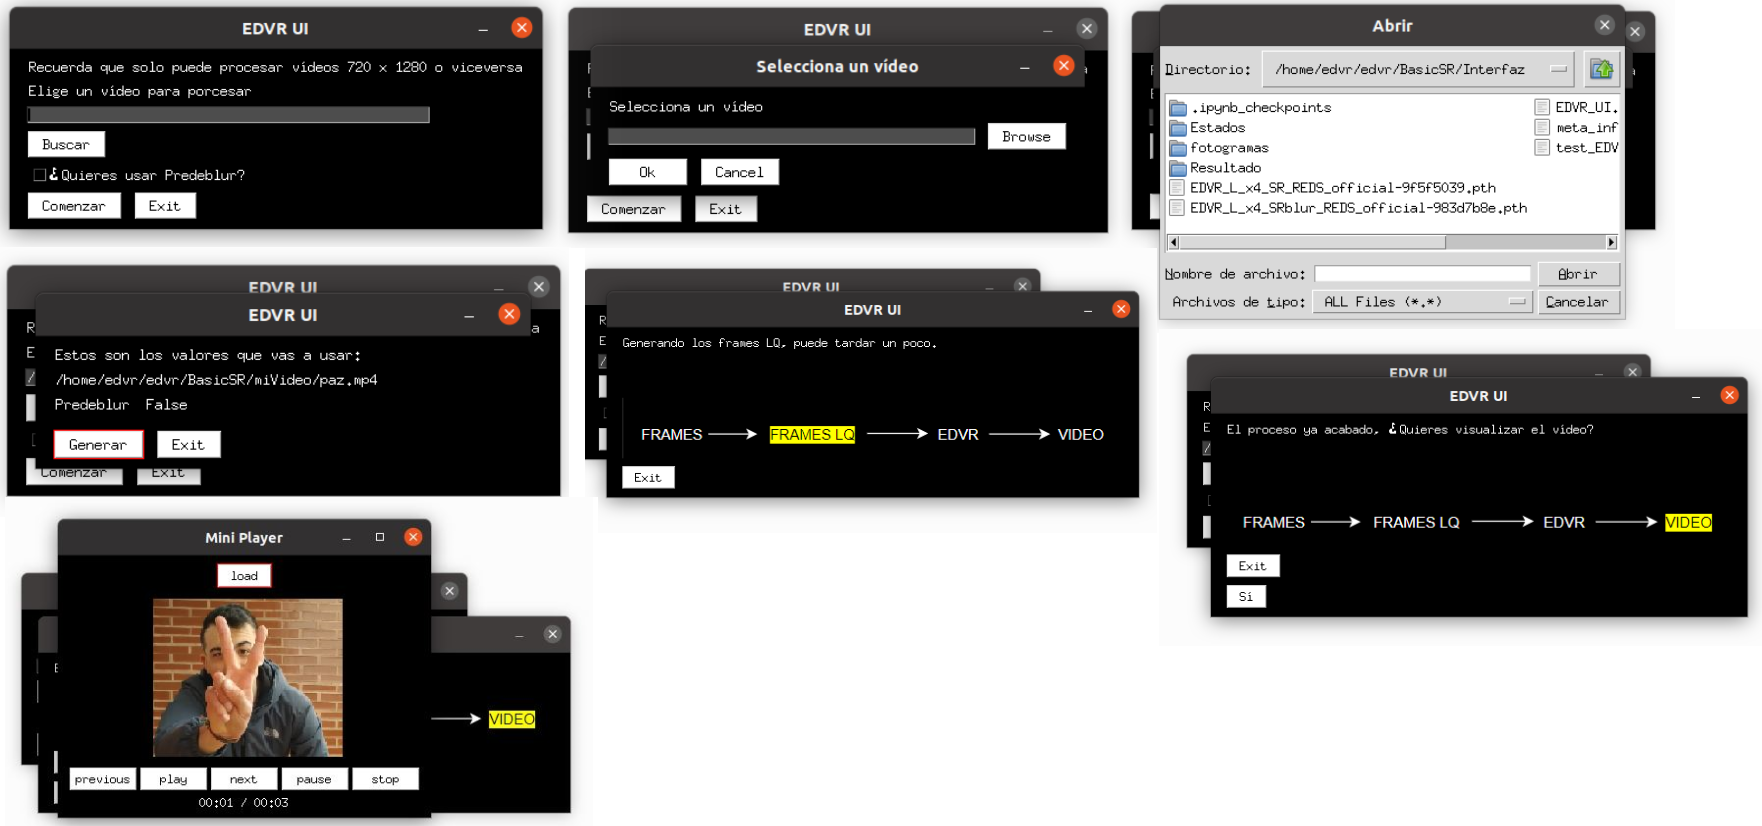
\includegraphics[width=1.1\textwidth]{finalvf}
		\caption{Pestañas de la interfaz durante la ejecución.}\label{1}
	\end{figure}
	\FloatBarrier



\bibliographystyle{plain}
\bibliography{bibliografiaAnexos}

\end{document}
